\chapter{Methods}
\section{Participants}
In the present study, we had a total population of 42 subjects, equally divided into two groups: 21 individuals were part of the healthy control group, whilst the remaining 21 were patients who suffered from a cortical or subcortical stroke. For what concerns the control group, the only criteria that had to be respected were the presence of a healthy neurological system and the command of Spanish, necessary for the response to behavioral questions. The recruitment for this group was made through several methods: in person, talking to alumni of the \href{https://www.experiencia.ub.edu/ca/}{Universitat de l'Experiència of Barcelona}, through personal contacts, and using the platform \href{https://www.sona-systems.com/}{Sonasystem}. \\
On the other hand, to recruit participants who experienced a stroke we used a database previously employed in another study made in the \href{https://brainvitge.org/}{Cognition and Brain Plasticity Unit} for movement rehabilitation with music therapy. Furthermore, we were also able to present our study at \href{https://www.fundacioictus.com/}{Fundaciò Ictus}, where we could select more participants. The exclusion criteria in both groups were: no visual or auditory impairments and no pregnancy.

Participants of the two groups were matched by age, where we can find a mean of 55,4 years old in the control group and of 56,4 for the stroke patients, with a non-significant difference (\textit{t} test: -0.299, \textit{p} value: .766). 
Likewise, the difference is gender didn't result significantly different (\textit{t} test: 1.56, \textit{p} value: .127), even though a majority of men in the stroke group and a preponderance of women in the control group could be observed. \\
Participants signed an informed consent before the experiment and they were reimbursed for their time. 
% This study was conducted according to the ethical rules presented in the General Ethical Protocol of the Faculty of Psychology and Educational Sciences.
% SD control: 8.291418397814637 SD stroke: 12.87041642867934

\section{Materials and methods}
The experiment was conducted with electroencephalography, precisely employing 64 electrodes, to capture the neural activity in the whole brain. The electrodes were attached to a cap, and connected to two amplifiers; to allow each electrode to transmit the signal we used a gel made of water and mineral salts. \\
The participants sat on a chair in front of the computer screen where the stimuli were presented and wore headphones to listen to the auditory stimuli, they were asked to avoid moving and blinking when the sensory stimuli were presented to avoid noise signal in the EEG recording. 

% This is a mix models study design presenting both auditory (footstep sound) and visual (walking point light figure) inputs Sensory inputs were presented at different frequency rates (1 Hz, 2 Hz, 3 6 Hz) in a rhythmic or random sequence, in three different experimental blocks i Auditory task ;;( Visual task ;;( Audiovisual task The experiment counts with 6 different conditions, presented 4 times in a randomized order.
The study design presented both auditory (footstep sound) and visual (walking point-light figure) inputs in a rhythmic or random sequence.
The stimuli adopted were of three different sensory kinds, which were assessed as the best to activate neural entrainment: there were visual, auditory and audiovisual stimuli. Such stimuli were previously used in a pilot study, only with healthy participants that aimed to discover at which frequency the stimuli presented were able to activate cerebral regions of interest that could integrate them. For such goal, in the previous research all the stimuli were played at different frequencies (1, 2, 3.6 Hz), whilst in the present one, they were only used at the frequency of 2 Hz, which appeared to be the best fitting one for neural entrainment. 

For what concerns the visual stimuli, a point-light figure walking, which represents the human body through white dots set in the primary joints of the body (Figure: \ref{fig: visual stimuli}), was used: it was created with \href{https://www.biomotionlab.ca/html5-bml-walker/}{BioMotionLab}, using a neutral subject, without any specific gender nor emotional display, and with average weight. After being created with the mentioned software, its frequency was adjusted to the desired one. The choice of a neutral point-light figure as the visual stimulus was made to focus only on brain activity elicited by movement processing frequency. Earlier studies have in fact shown that the presence of different important biological and social features that can be inferred from figures may enhance and grab other processes not primarily related to movement perception \parencite{Cracco_2022}. \\
For the audio stimuli, the sound of footsteps at 2Hz with a neutral connotation was used (Figure: \ref{fig: audio stimuli}). Finally, the audiovisual stimuli were a union of the point-light figure walking and the sounds of the footsteps associated with it. 
\begin{figure}[h]
    \centering
    \begin{subfigure}[h]{0.4\textwidth}
        \centering
        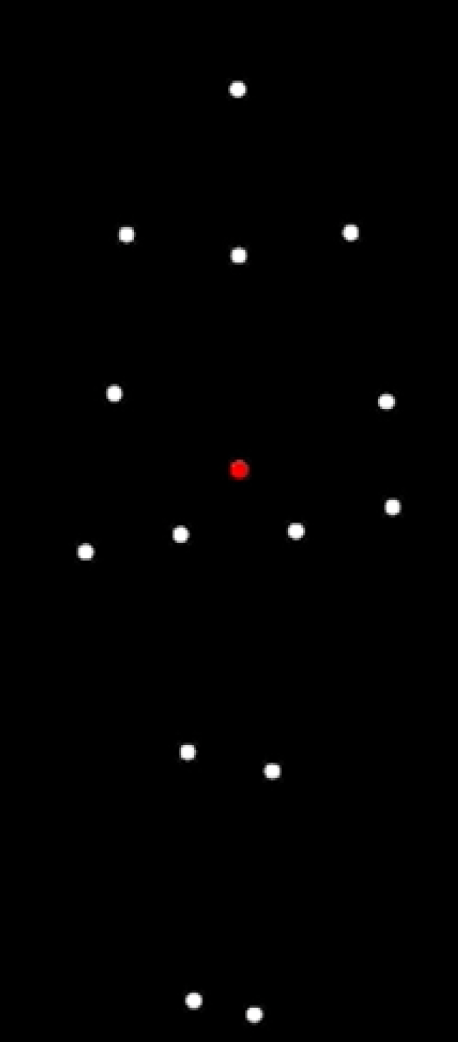
\includegraphics[width=0.35\textwidth]{appendix/point_light_figure.png}
        \caption{Point-light figure used for visual condition}
        \label{fig: visual stimuli}
    \end{subfigure}
    \hspace{4em}
    \begin{subfigure}[h]{0.4\textwidth}
        \centering
        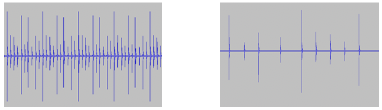
\includegraphics[width=0.85\textwidth]{appendix/audio_images.png}
        \caption{Rhythmic and random audio stimuli}
        \label{fig: audio stimuli}
    \end{subfigure}
    \label{fig: stimuli}   
\end{figure} \\
During the EEG experiment between each stimulus, six behavioral questions were presented on the display \ref{fig: Behavioral questions}: they referred on how the participant felt while seeing the point-light figure walking or listening to the footsteps (e.g. if they felt relaxed or involved with the movement). The questions had to be answered on a Likert scale with values between 1 (strongly disagree) to 5 (strongly agree), using the keyboard positioned in front of the subjects. 

Before executing the electroencephalography, we also sent via e-mail a questionnaire, whose goal was to measure the level of physical activity of each participant, which would be later correlated to the EEG results, to see if it could influence neural activity. \\
We used the \textit{Active-Q} questionnaire, which was created to assess the total physical activity and inactivity in adults, through a series of multiple choice questions (referred to a one-year time) on daily activity, mean of transportation used, leisure and sports activities; and the time a day spent for each of them \parencite{Bonn_2012}. 
The questionnaire was translated in Spanish from the original English version and transformed from a PDF file into an interactive digital version using the platform \href{https://www.qualtrics.com/uk/?rid=ip&prevsite=en&newsite=uk&geo=ES&geomatch=uk}{Qualtrics}. 

\section{Procedure}
%% If you did an experiment detail here how it was. Space, number of sessions
Our study consisted of three different blocks, each one with one type of stimuli previously described (visual, audio or audiovisual). 
Each of the stimuli lasted 60 seconds and was repeated eight times in all the blocks, differentiated by four conditions: synchronicity and asynchronicity, which will be a key element for our analysis; and the number of variations used as a focus tool. These refer to the changes of the pitch (to a more acute or grave sound) in the sound stimuli and the switch of color  in the central point of the point-light figure (from red to white) in the visual and audiovisual stimuli. Such changes were introduced as an attentional task for the participants: they had to count and tell the experimenter how many changes they were able to observe or hear at the end of each stimulus, through a speaker. \\
The four conditions related to each stimulus were presented twice, in a random order. 

The experiment was structured with the software \href{https://pstnet.com/products/e-prime/}{E-prime}, which allowed us to build an experiment with different stimuli presentations (e.g. adding images, questions and text). \\
We indeed included the instructions text at the beginning and later a white fixation cross before the start of each stimulus, which lasted five seconds and gave time to the participant to prepare and relax; on the other hand, a blue fixation cross was displayed during the audio stimuli to keep the eyes of the participants open and fixed. \\
As mentioned before, after each one of the eight stimuli, we showed six behavioral questions and afterwards a figure of an eye-blink, which lasted fifteen seconds and allowed the participant to blink if needed.

Individually the blocks lasted approximately fifteen minutes (depending on how long the participants would take to answer the behavioral question) and a break of roughly five minutes was taken between all blocks to fix the conductivity of the electrodes with the gel and to let the participants rest. Altogether, the experiment and its preparation had a duration of almost two hours.

\section{Analysis}
%% ---- EEG analysis part
The EEG data was registered through the software provided by \href{https://brainvision.com/applications/brain-vision-software/}{BrainVision} at the sampling rate of 1000 Hz; for all the subjects we made three different registrations one per condition determined by the stimuli (visual, audio, audiovisual). \\
Before the actual frequency tagging analysis, the data was preprocessed: all the chunks of register that weren't necessary (i.e. the initial part with the instructions, the one related to the eye-blink figure and the ones corresponding to the behavioral questions) were trimmed. Later we re-referenced the data to channels 31 and 32, which indicate the electrodes TP9 and TP10, positioned on the mastoids. Finally, we ran the Independent Component Analysis to remove artifacts and saved the preprocessed data into a new file. 

After the data for every block for all the participants was preprocessed, we started the analysis with the help of some scripts made for the previous study adjusted according to our necessities. \\
Firstly, we extracted the epochs from the processed data: epochs of 20 seconds were obtained from the 60 seconds of each stimulus using the method of surface Laplacian (Claudio, 2015). Secondly, from the files just generated, we created \href{https://www.fieldtriptoolbox.org/}{FieldTrip} files, that allow to perform analysis in time and frequency domains to study oscillatory brain activity and its modulation over time. We then proceeded to apply the Fast Fourier transform (FFT) on each condition (visual, audio and audiovisual) and in the two different cases (synchronicity and asynchronicity, also referred to as rhythmic and random), therefore six variables were obtained. \\
Using these variables we created the desired graphs, showing how the activity power would change through conditions, cases and channels in order to see if we could find peaks of activity correspondent to the frequency used for the stimuli. 
% Four different graphs for distinct channels: one representing the grand average, one for the z-scores for the grand average, one showing Signal-to-Noise Subtraction (SNS) or Baseline Subtraction and the last one depicting the Averaged Signal-to-Noise Ratio (SNR). 

Finally, our analyzed data was utilized to create the desired topographies, both two-dimensional and 3D, showing the cerebral activity for each sensory stimuli, divided into rhythmic and random conditions, adding the ones to represent the difference between these two. In the two-dimensional topographies we decided to distinguish the electrodes corresponding to the different regions of interest coloring them in white.\\
The analysis just described, including all the graphs and images was made separately for the control group and stroke patients populations. 

%% ---- behavioral questions analysis part 
Meanwhile, for what concerns the analysis of the behavioral questions, we searched for all the answers given by the participants, which were collected into a .txt file by E-prime through a Python script. This would insert each numeric answers into an Excel file, so that later it could be used for statistic operations. \\
For each question of every stimulus, specifically differenced into rhythmic and random, and population group we calculated its average, median, standard deviation, and significance through a Wilcoxon Signed-Rank test if the data resulted non-normally distributed, and a paired T-test if it resulted otherwise. In order to understand the distribution of every set of data we earlier performed the Shapiro–Wilk test. \\
We inserted all of our numerical results into different tables and build various bar plots to show graphically the results for each condition and group, to have a clear visual comparison between the rhythmic and random condition. Finally, we decided to achieve two additional statistical analysis: one for the mean of all the questions of the different stimuli just to compare the rhythmic and random condition, and the other one with the same mean but for the two distinct population groups so that the difference between these two could be observed. 

%% ---- questionnaire analysis part 
Regarding the Active-Q questionnaire we conducted the analysis following the instruction reported on the article where its efficiency \parencite{Bonn_2012}. Initially, we exported in an Excel file the results collected by Qualtrics with their numeric values (e.g. if the participant had selected the first option, the result would have been 1), this was imported in a Python file where the numeric values related to each activity were transformed into the MET values reported in the table \ref{fig: met_values} that were encountered in the previously cited article. On the other hand, the frequency of each activity was measured multiplying the hours/minutes a day, if necessary calculating the average if a range of time was present and converting them to hours (e.g. 15-29 minutes was converted to 0.36 h) for the number of days per week.  \\
After creating an Excel table with the new values accorded with MET values and the duration of hours/week, we proceeded to calculate the final Active-Q value, which returns a number of kilojoules per day, using the following formula: 
\[
\text{EE}_{\text{activity}} \, (\text{kJ/day}) = \text{MET}_{\text{activity}} \cdot \text{Weight} \, (\text{kg}) \cdot \text{Duration}_{\text{activity}} \, (\text{h/d}) \cdot 4.184
\]
The MET value and duration of the activity were multiplied by the weight of each participant (which was asked individually to the participant before the experiment), and the number 4.184, which is a conversion factor used to transform values from kcal to kJ. The obtained results represented the daily physical activity of each participant. The physical activity was later correlated with the brain power registered through EEG to see if it could influence the neural entrainment observed. 

In order to obtain a numerical value for each participant and condition representing the neural activity experienced perceiving the different stimuli, we proceeded to extract the power spectrum density of the most active electrodes in the different condition and population group. For what concerns the control group the ones taking into account were: TP7 and T8 for the audio condition, TP7 and O1 for the audiovisual one, and finally just O1 for the visual condition. The electrodes with the highest power density slightly changed in the stroke population, where we took in consideration FC5, TP7 and T8 for the audio stimuli; TP7 and Oz for the audiovisual and Oz for the visual condition. 

Once we had these values we could proceed to correlate for each participant of the different groups their physical and brain activity; as well as their brain activation and their answers to our behavioral questions, in order to see if the involvement and enjoyment of the stimuli could influence individual neural entrainment. \\
To represent such correlations we built different scatter plots for each population group and calculated Pearson's correlation coefficient and its relative \textit{p} value.